 \chapter{Verger n\textdegree2}
 \label{chap:bloc2}
 
 On présente ici le dispositif présent sur le verger expérimental n\textdegree2 ainsi que les dynamiques d'inflorescences et de larves obtenues grâce aux données des relevés effectués sur cette parcelle.
 
 Le dispositif mis en place était similaire à celui du verger n\textdegree1, à la différence de l'ordre des modalités de couverture du sol (voir figure~\ref{fig:schema2}).
 
 \begin{figure}[ht]
 \centering
 
 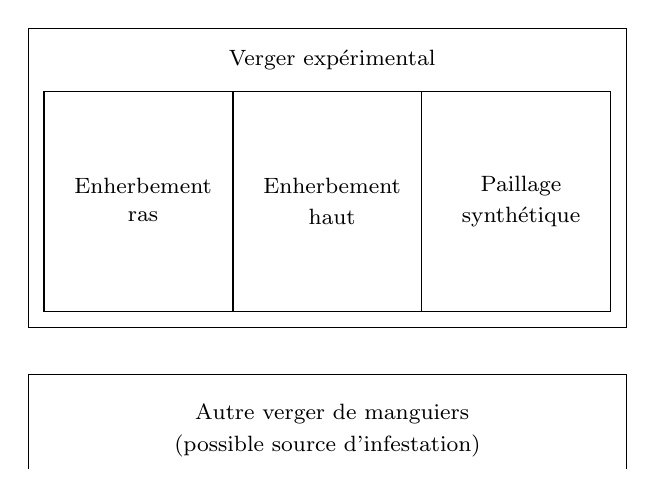
\begin{tikzpicture}[scale = 0.4]
  \draw (0,5) rectangle (18, 12);
  \draw (6, 5) -- (6, 12);
  \draw (12, 5) -- (12, 12);
  \draw (-0.5, 0) -- (-0.5, 3) ;
  \draw (-0.5, 3) -- (18.5, 3) ;
  \draw (18.5, 3) -- (18.5, 0);
  \draw (9, 1.75) node{\text{ \footnotesize Autre verger de manguiers}};
  \draw (9, 0.75) node{\text{\footnotesize (possible source d'infestation)}};
  \draw (9, 9) node{\text{ \footnotesize Enherbement}};
  \draw (9, 8) node{\text{ \footnotesize haut}};
  \draw (3, 9) node{\text{ \footnotesize Enherbement}};
  \draw (3, 8) node{\text{ \footnotesize ras}};
  \draw (15, 9) node{\text{ \footnotesize Paillage}};
  \draw (15, 8) node{\text{ \footnotesize synthétique}};
  \draw (-0.5, 4.5) rectangle (18.5, 14);
  \draw (9, 13) node{\text{ \footnotesize Verger expérimental }};
 \end{tikzpicture}
 \caption{Schéma de l'expérimentation menée. Le verger sur lequel ont été testées les trois modalités de couvertures du sol était situé à côté d'un autre verger. Bien que cet autre verger n'avait pas de rôle particulier, il a probablement servi de source d'infestation exogène au verger expérimental.}
 \label{fig:schema2}
\end{figure}
 
 Le verger n\textdegree2 présente des caractéristiques particulières, rajoutant des différences supplémentaires entre les différentes sous-parcelles, en plus des différentes modalités.
 Ce verger est disposée «en escalier», avec une modalité sur chaque «marche».
 L'ensoleillement n'était pas le même entre les différentes modalités, et cela se ressent sur la figure~\ref{fig:inflos2}.
 La sous-parcelle avec un paillage synthétique --- la plus ensoleillé --- présente ainsi plus d'inflorescences que les deux autres.
 On retrouve aussi des différences d'inflorescences entre les parcelles enherbées, celle avec l'enherbement haut avait plus de soleil que l'autre, et elle a eu plus d'inflorescences.
 
 \begin{figure}[ht]
\centering
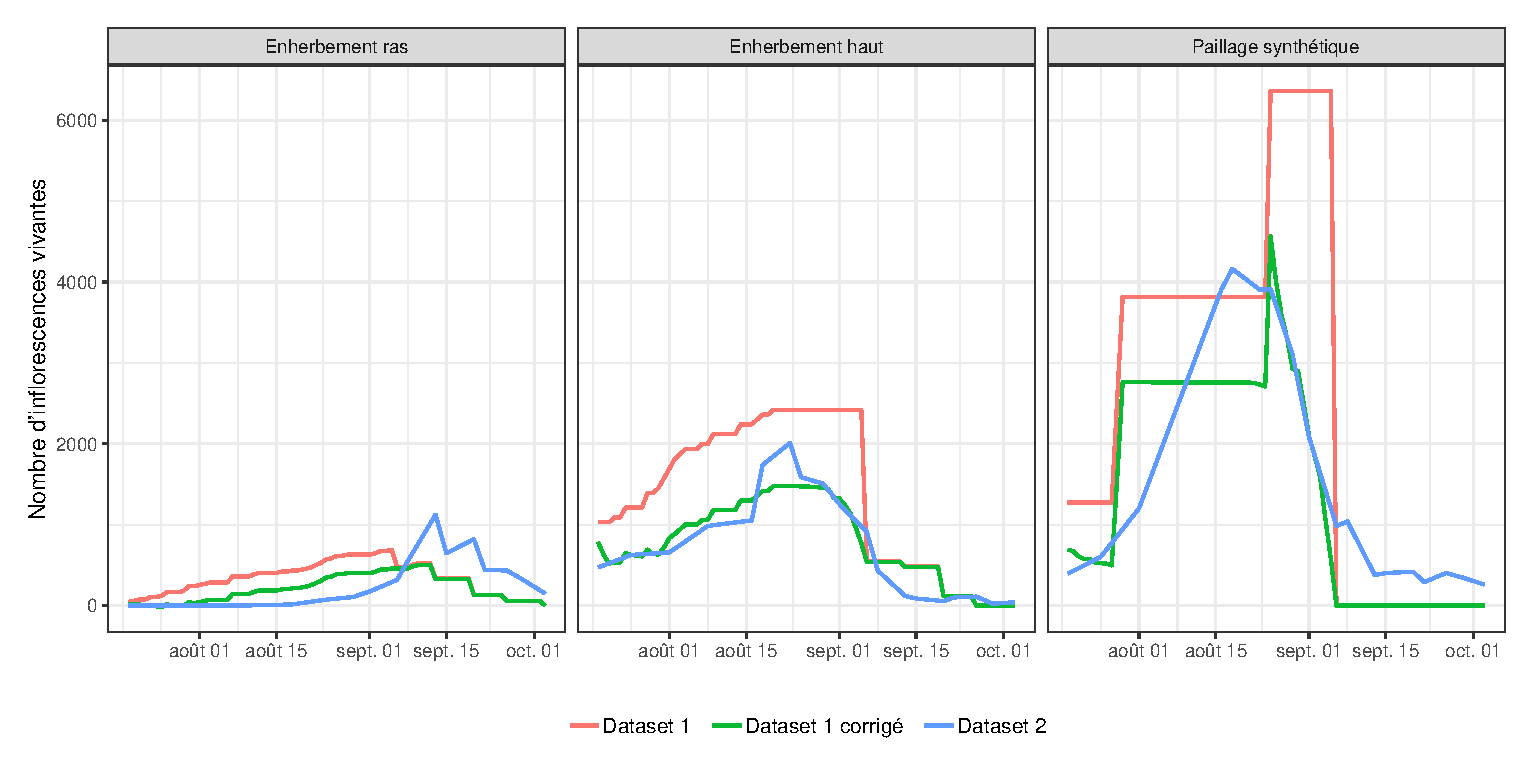
\epsfig{file = r/inflos2.eps, scale = 0.59}
\caption{Comparaison des différentes dynamiques d'inflorescences vivantes du verger n\textdegree2 en fonction du \emph{dataset} utilisé. Même après correction, on observe des différences entre les dynamiques issues des différents jeu de données, en particulier pour les deux premières modalités.}
\label{fig:inflos2}
\end{figure}
\newpage
 On peut noter aussi des différences entre les deux jeux de données. C'est flagrant pour la modalité «paillage synthétique», où il n'y a seulement que 5 observations dans le \emph{dataset 1} produisant cette dynamique particulière. À cela se rajoute la variabilité du phénomène donnant des dynamiques très différentes pour des échantillonnages différents. Seule la sous-parcelle avec un enherbement haut présente des dynamiques similaires entre les deux jeux de données.
 
 Les dynamiques de larves pour ce verger sont visibles sur la figure~\ref{fig:larves2}.
 
 \begin{figure}[ht]
\centering
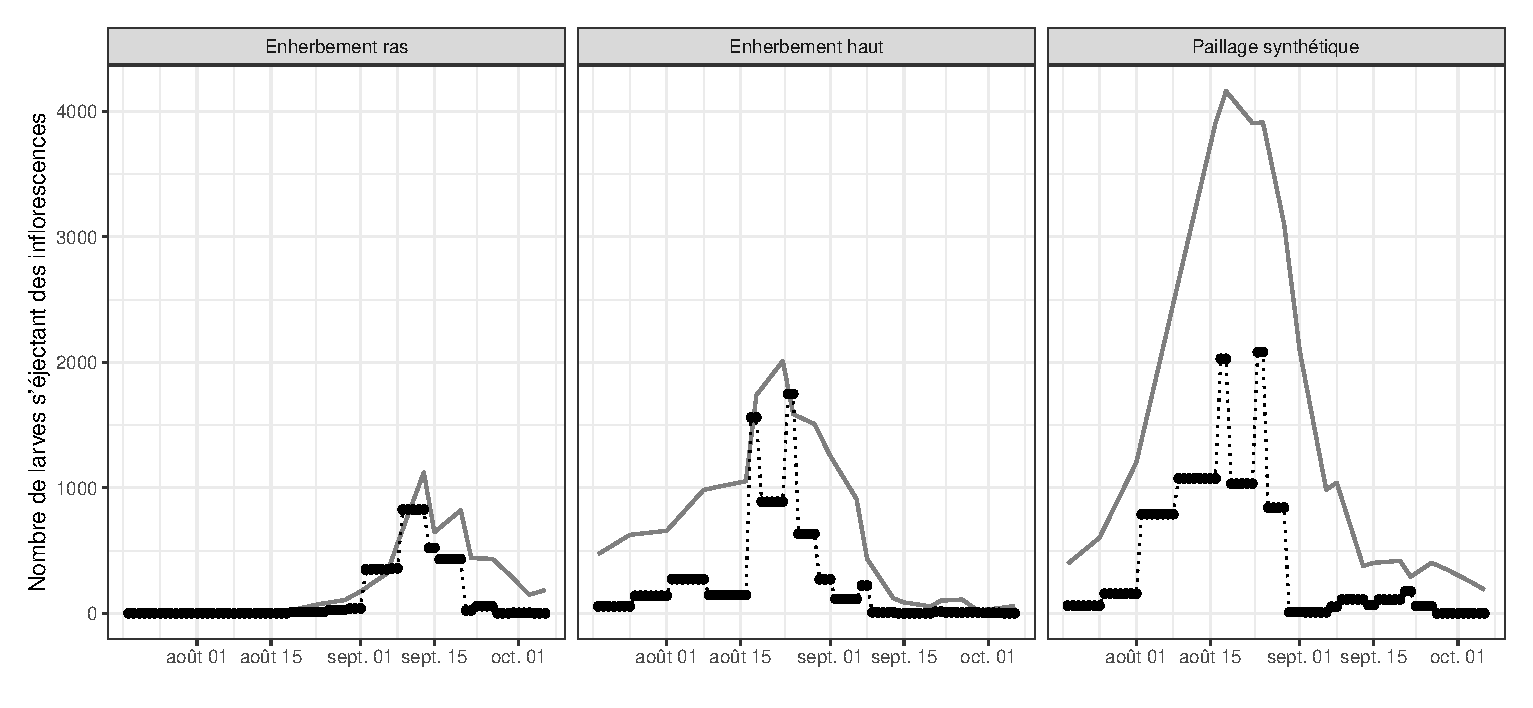
\epsfig{file = r/larves2.eps, scale = 0.59}
\caption{Dynamiques de larves s'éjectant des inflorescences des manguiers chaque jour dans le verger n\textdegree2 pour chacune des trois sous-parcelles. En gris sont visibles les dynamiques d'inflorescences vivantes (issues du \emph{dataset 2}, $I^2_t$).}
\label{fig:larves2}
\end{figure}

